\section{Angular dependency of the Rutherford cross section}
The Rutherford differential cross section \parencite[p. 16]{noteBB} is given by
\begin{align}
    {\left( \diff[d]{\sigma}{\Omega} \right)}_|Rutherford| =
    {\left(\frac{Z_1Z_2 e^2}{4E_{\infty}} \right)}^2
    \frac{1}{{{\sin}^4(\frac{\theta}{2})}},
\end{align}
where $Z$ is the proton number of each interacting particle, $E_{\infty}$ is
the asymptotic energy, and $\theta$ is the scattering angle. If the energy is
in units of $\si{\mega\electronvolt}$, this differential cross section will be in units
of $\si{\milli\barn\per\steradian}$.
This formula neglects the recoil energy of the target, which will be discussed
later on. 

%% %%

As mentioned earlier, the experimental setup uses a Faraday cup to meassure the
incomming particle flux. What is really meassured is the amount of
non-scattered particles. Since this is a very large number relative to the amount of scattered
particles, the number of incomming particles can be assumed to be the number of
detected particles within the Faraday cup.

The number of detected events, $\mathrm{d}N$ is assumed to follow a Poisson
distribution, such that the statistical uncertainty of this number is the
square root of the sum, $\sigma_|dN| = \sqrt{\mathrm{d}N}$

This count number is read off the collector. The collector counted $10^{11}$
counts per coulomb, and as there are $6,24150913\ \cdot10^{18}$ elementary
charges per coulomb, we can related the count number to an amount of detected
protons, $N$.

The number of particles, $\mathrm{d}N$, scattered off a thin target of nuclei density
$n_|tar|$ and thickness $dx$, and emerged into a small solid angle
$\mathrm{d}\Omega$ in a certain timed interval, is detected in a Silicon
detector, and the relation of these sizes are:
\begin{equation}
    \mathrm{d}N = N n_|tar| \mathrm{d}x \mathrm{d}\Omega,
    \diff[d]{\sigma(\theta,\phi)}{\Omega}.
\end{equation}

\subsection{Meassurements}
To test the angular dependency of the Rutherford cross section, the Silicon
detector is set at a variable angle.

As mentioned earlier, the target has two layers, and thus the incomming beam of
ions can scatter on both gold and carbon. As the Rutherford scattering is a
coulomb interaction, we expect the gold layer to scatter the most at higher angles.

This is recognized when comparing with data, which is not a simple gaussian
distribution. This is a consequense of a double layered target, such the
incomming hydrogen ion will scatter of both Carbon and Gold. Fitting a double
gaussian, one gather six parameters. Amplitude, centroid and standard deviation
of both gaussians. Here we use the linear combination of the two scattering
processes. 

Notice that the gaussian of greatest amplitude is corresponding to gold, which
is in agreement with the relative sizes of the two atoms. Stable isotopes of
gold has a nuclear number of $A_|Au| = 197$ whereas carbon has $A_|C| = 12$.

What is interesting is how the two peaks change relative position as a
function of scattering, merging their gaussian distribution at low angles, and
seperating at higher angles.

%\begin{figure*}
%\centering
%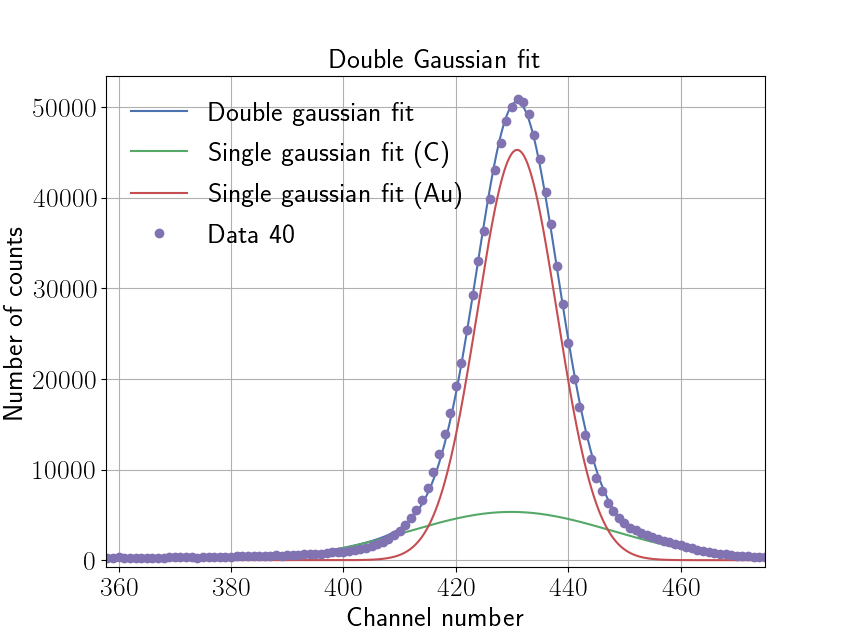
\includegraphics[width=0.99\columnwidth]{Data_40}
%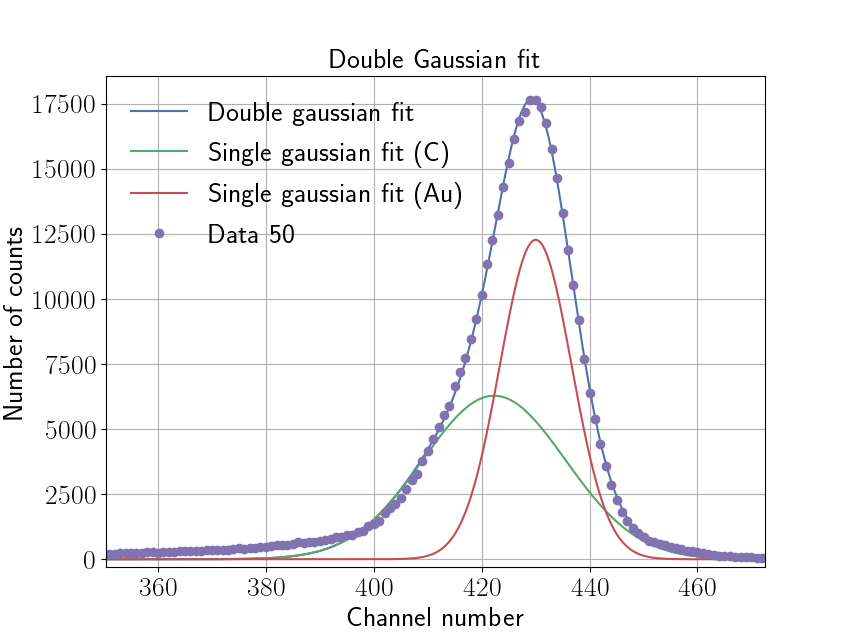
\includegraphics[width=0.99\columnwidth]{Data_50}
%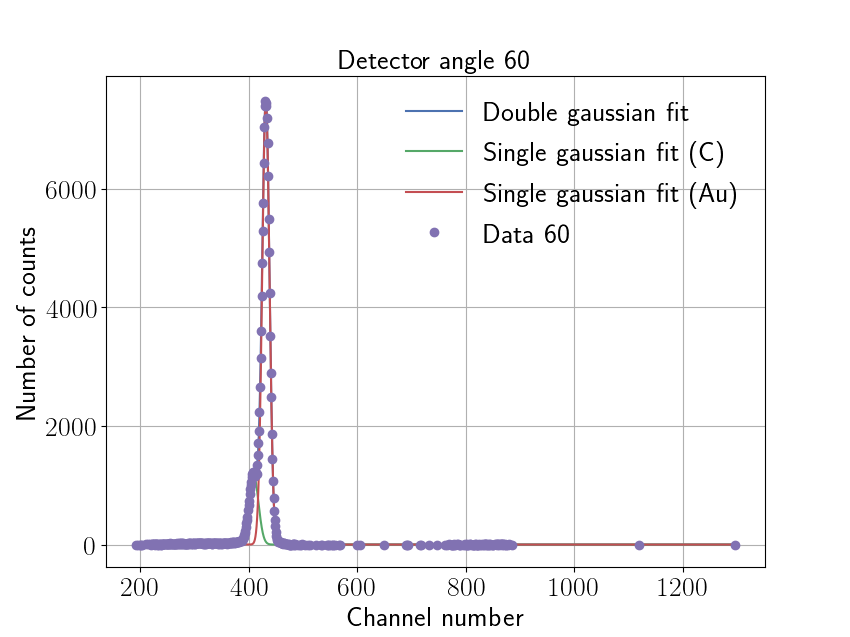
\includegraphics[width=0.99\columnwidth]{Data_60}
%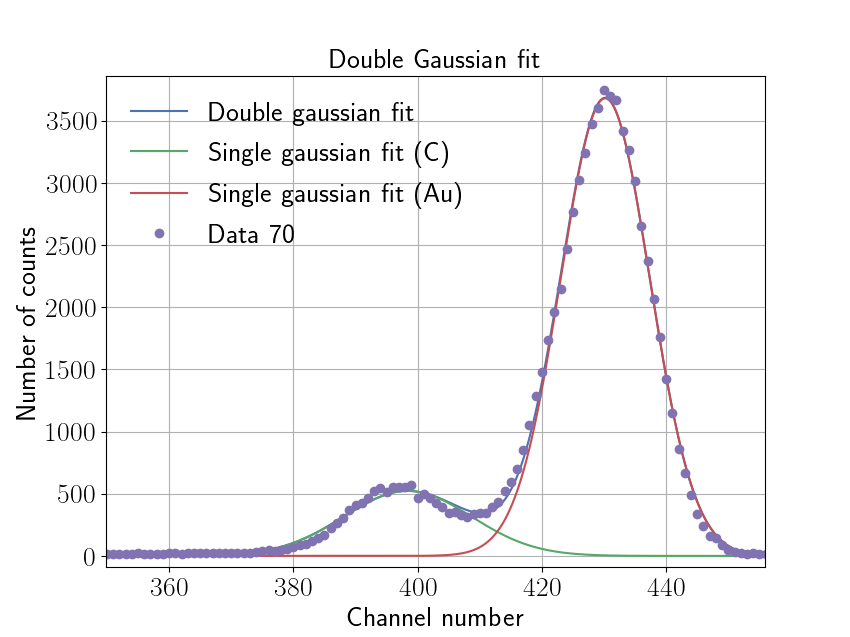
\includegraphics[width=0.99\columnwidth]{Data_70}
%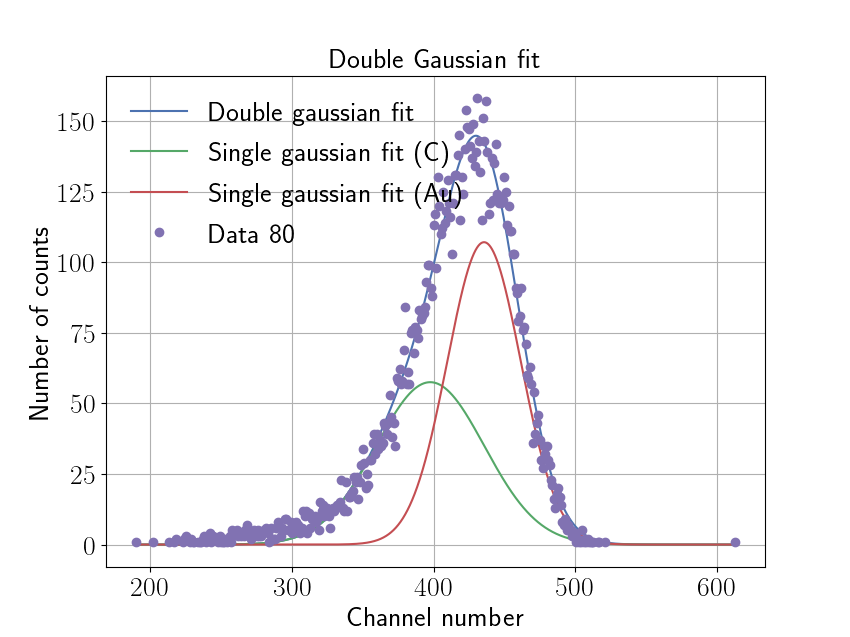
\includegraphics[width=0.99\columnwidth]{Data_80}
%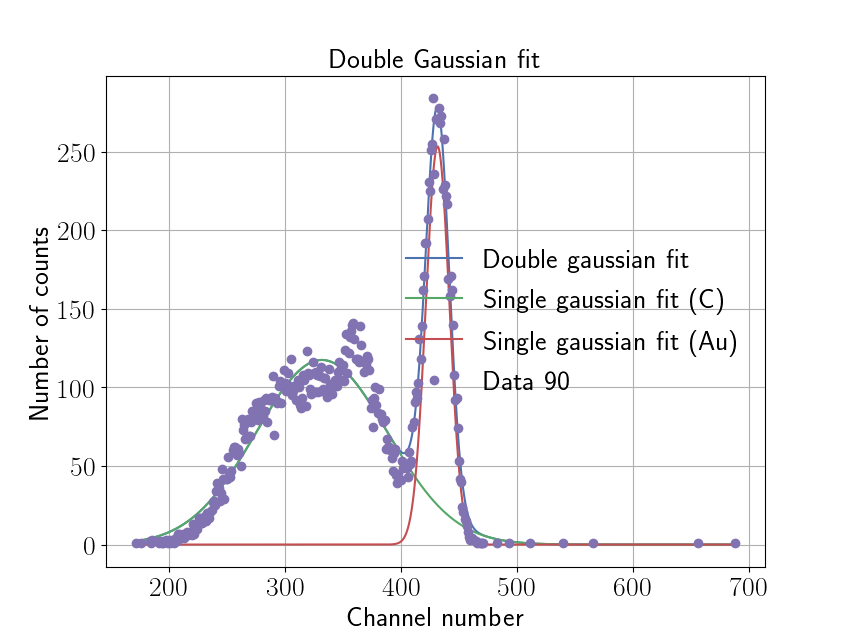
\includegraphics[width=0.99\columnwidth]{Data_90}
%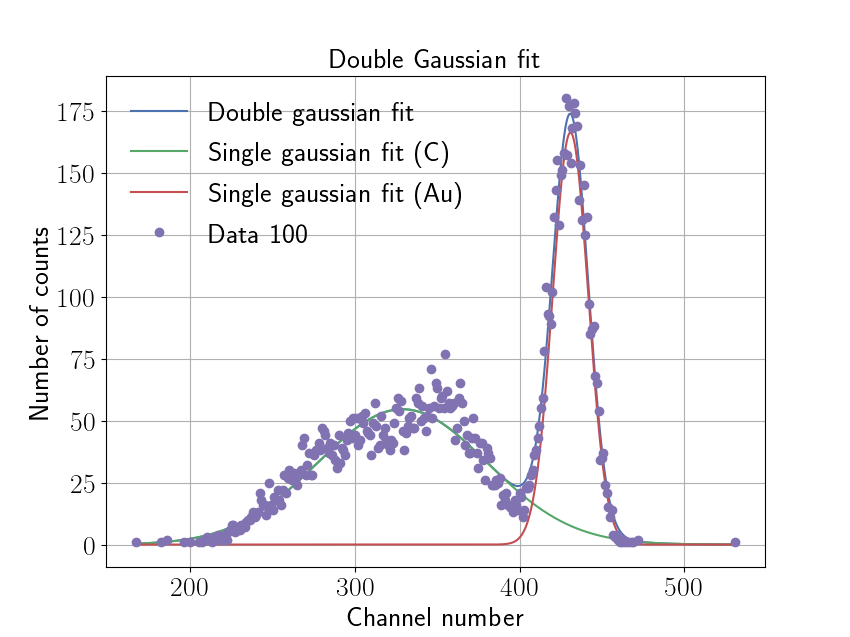
\includegraphics[width=0.99\columnwidth]{Data_100}
%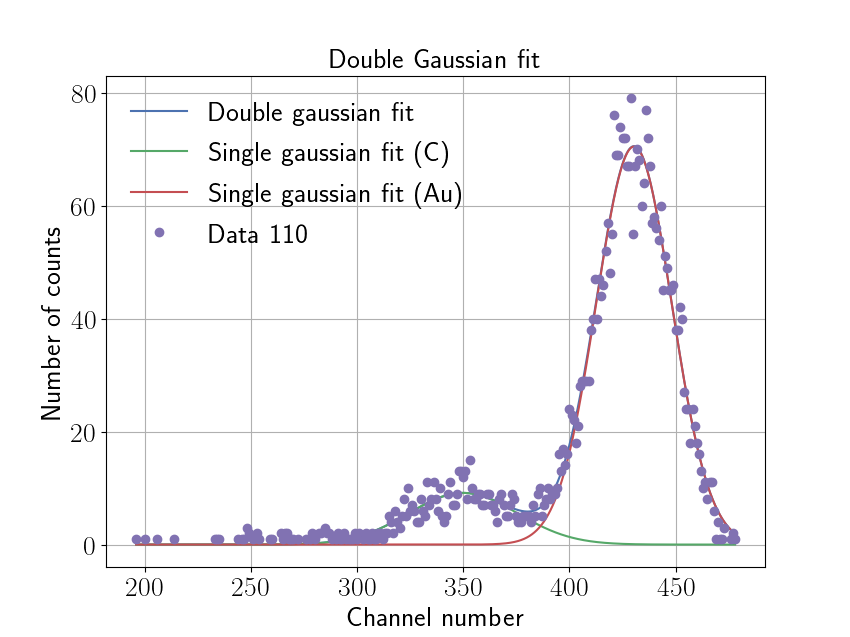
\includegraphics[width=0.99\columnwidth]{Data_110}
%\label{fig_angular_dependency}
%\end{figure*}
%
%\begin{figure*}
%    \centering
%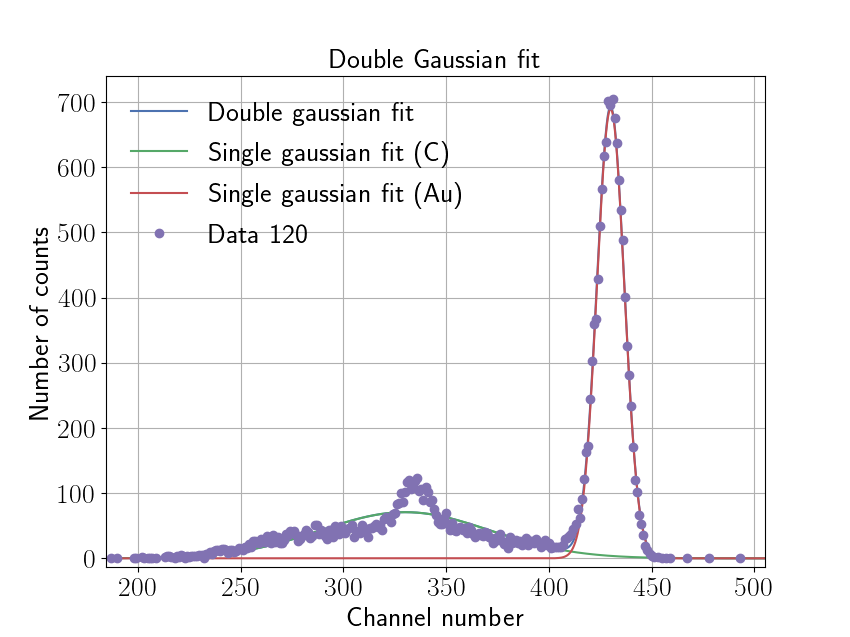
\includegraphics[width=0.99\columnwidth]{Data_120}
%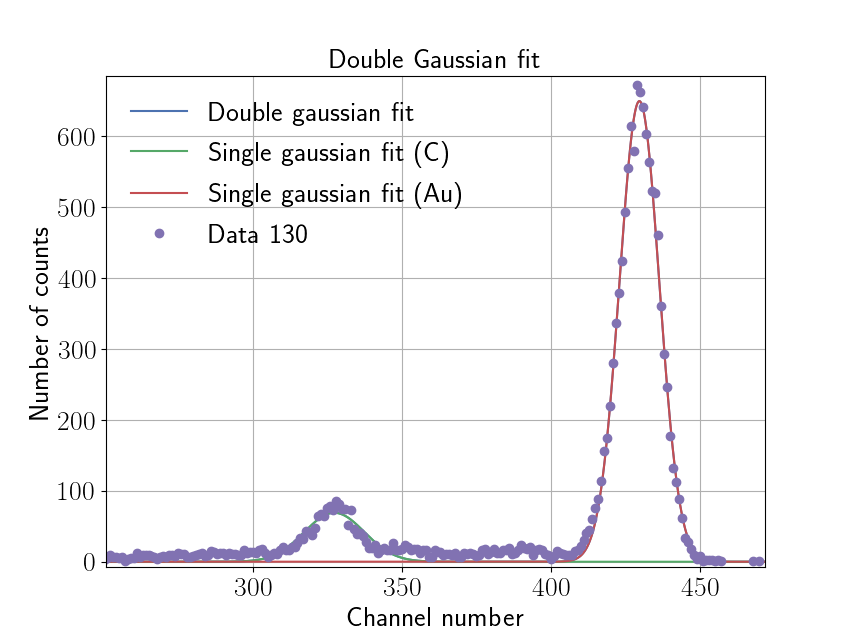
\includegraphics[width=0.99\columnwidth]{Data_130}
%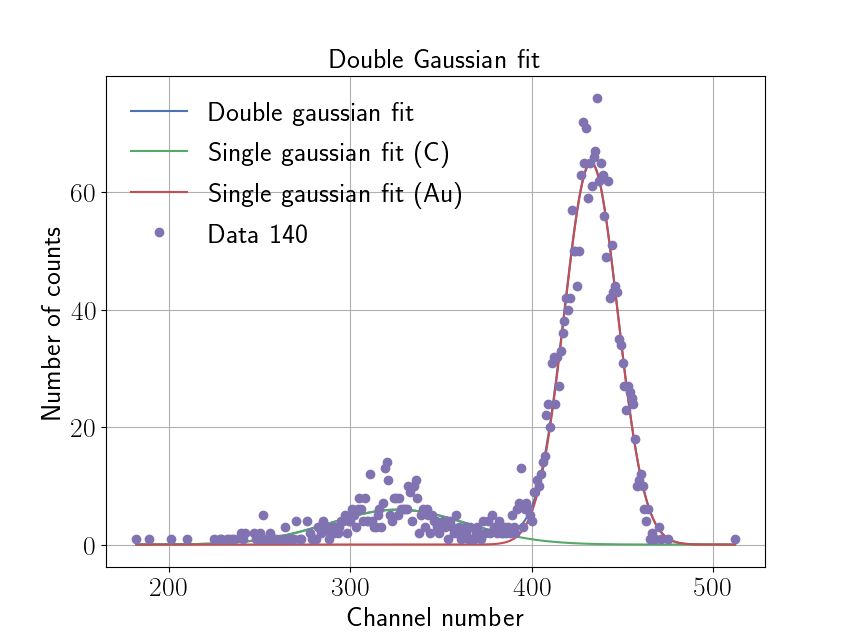
\includegraphics[width=0.99\columnwidth]{Data_140}
%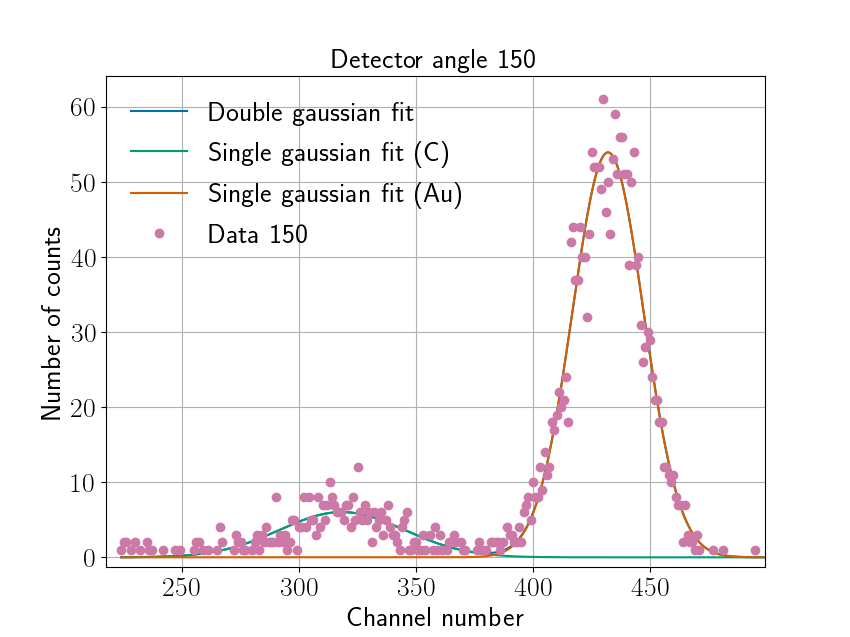
\includegraphics[width=0.99\columnwidth]{Data_150}
%\label{fig_angular_dependency2}
%\caption{Angular dependency}
%\end{figure*}


\begin{figure}[h]
	\centering
		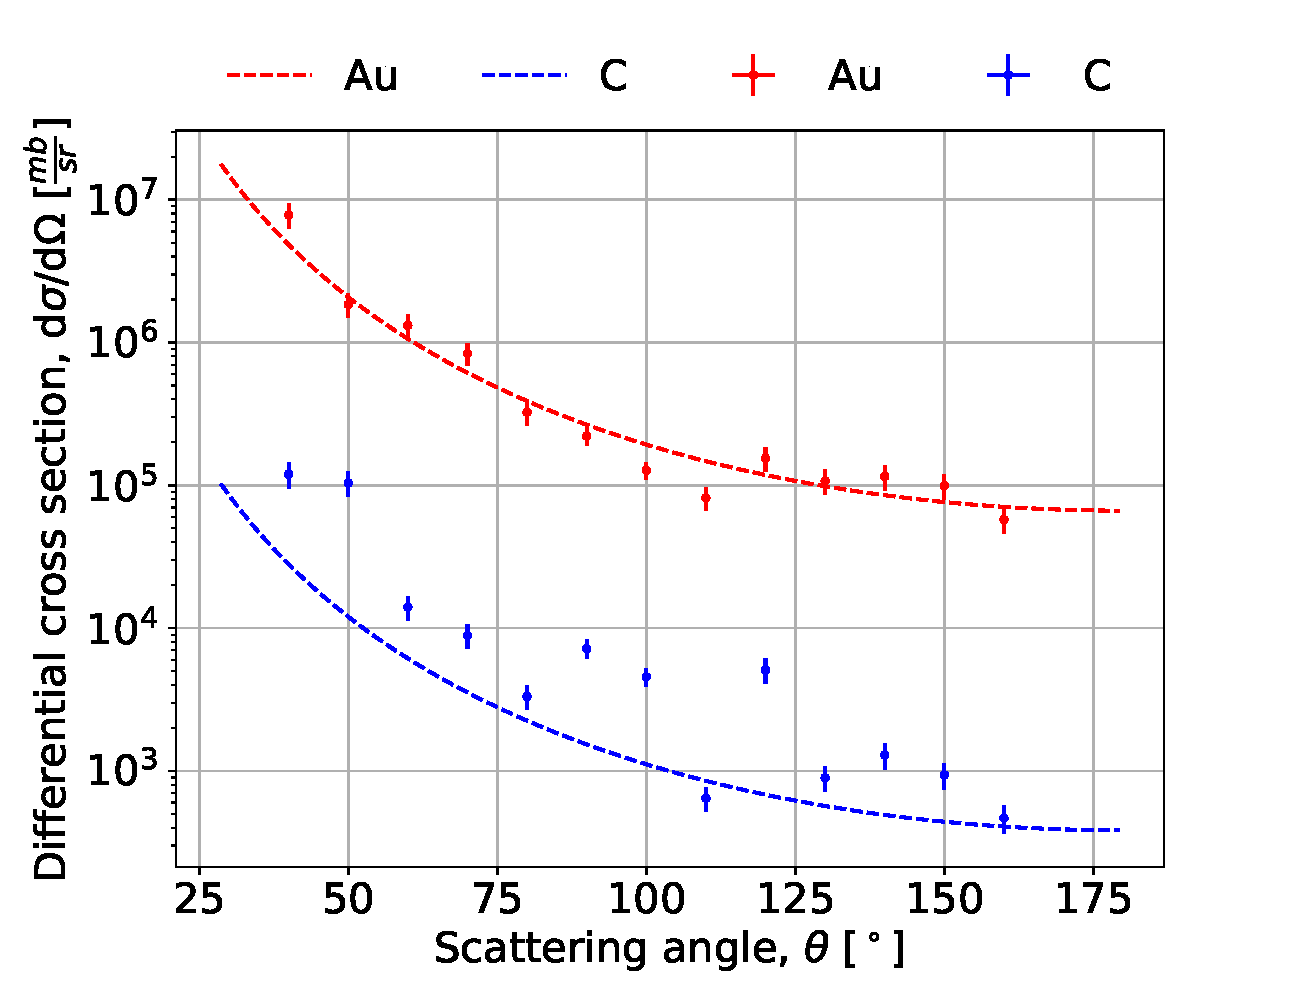
\includegraphics[width=0.45\textwidth]{Differential_cross_section.eps}
	\caption{bb}
	\label{fig:Differential_cross_section}
\end{figure}

Using the calibration to convert the centroid channel number of each gaussian,
we can plot the energies as a function of scattering angle.

\begin{figure}[h!]
\centering
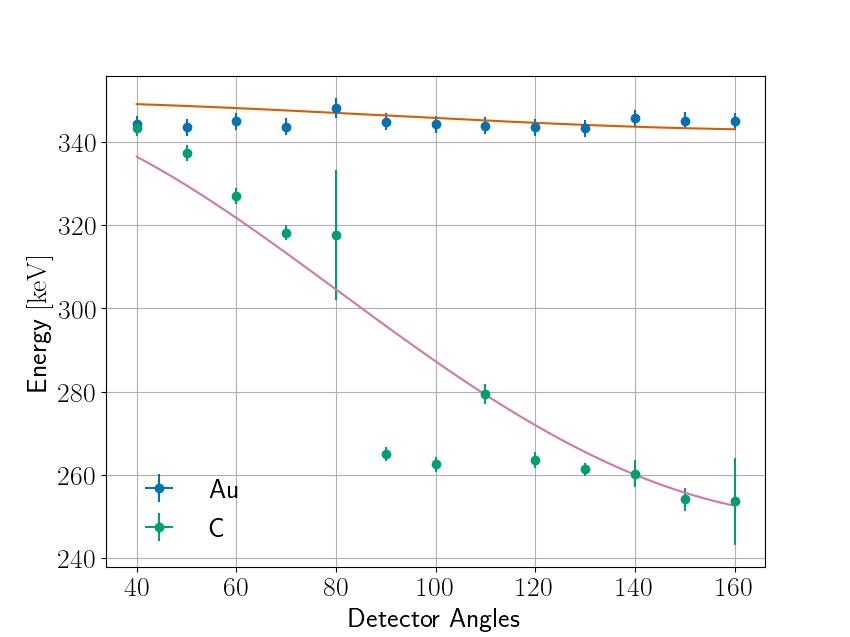
\includegraphics[width=0.99\columnwidth]{fig_energy}
\caption{Energies of Carbon and Gold scattered compared to theoretical
function.}
\label{fig_energy}
\end{figure}




\newpage
